\documentclass[12pt]{article}
\usepackage{../../template}
\title{Lecture 3}
\author{niceguy}
\begin{document}
\maketitle

\section{Instead of guessing...}

Based on our current model, it is difficult to solve circuits with diodes, because we have to split into cases. Using a different model \ref{diode}...

\begin{figure} \label{diode}
    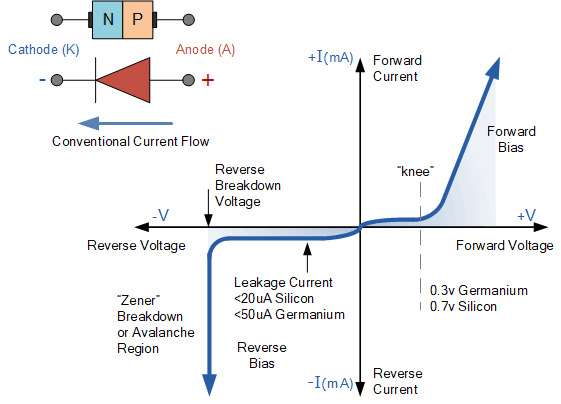
\includegraphics[width=\textwidth]{diode.jpg}
    \caption{Forward and Negative Biases of Real Diodes}
\end{figure}

\begin{itemize}
    \item $V$ and $I$ have a nonlinear relation (one increases with the other)
    \item Until 0.7V is reaches (for silicon), current is very low
        This point is called the knee
    \item The region beyond 0.7V is called the forward bias
    \item At a negative voltage, there is a leakage current that is more or less constant, $<20\unit{\mu A}$ for silicon
    \item At reverse breakdown voltage, there is an "avalanche" region, where current decreases (further from 0) rapidly
\end{itemize}

We approximate the relation with

\begin{equation}
    I = I_S \left(e^{\frac{V}{V_T} - 1}\right)
\end{equation}

where $I_S$ is the saturation or scaling current, and $V_T$ the thermal voltage, where

\begin{equation}
    V_T = \frac{k_BT}{q}
\end{equation}

On the positive end, when $V >> V_T$, we approximate

\begin{equation}
    i \approx I_Se^{\frac{V}{V_T}}
\end{equation}

\textit{Note: we can of course use a Taylor approximation, but at small V, the diode is essentially off anyway.}

\begin{ex}
    Consider a simple circuit with a voltage source $V_{DD}$, resistor, and diode (forward bias). Current across diode is

    $$I_D = I_Se^{\frac{V_D}{V_T}}$$
    substituting into the resistor,
    $$I_D = \frac{V_R}{R} = \frac{V_{DD}-V_D}{R}$$
    Eliminating $V_D$ gives the transcendal equation
    $$I_D = \frac{V_{DD} - V_T\ln\left(\frac{I_D}{I_S}\right)}{R}$$
    Inventing values and comparing it with the solution according to the first model
    $$I_D = \frac{V_{DD}}{R}$$
    We let the diode be 0.7V at 1mA and $V_T$ be 25mV. Plugging, we find $I_S = 6.9 \times 10^{-16}\unit{A}$. Solving gives us
    $$I_D = 4.264 \unit{mA}, V_D = 0.736\unit{V}$$
\end{ex}

\end{document}
